\section{Sensitivity Analysis}

\setlength{\parskip}{0.7em}
\setlength{\parindent}{0pt}

We use a one-at-a-time sensitivity analysis around the recommended frontier point, varying one parameter at a time while holding all others fixed.

The current analysis uses two stages:
\[
\mathcal{M}_{\mathrm{screen}} = \{0.5,\;2.0\},
\qquad
\mathcal{M}_{\mathrm{full}} = \left\{0.5,\;0.75,\;1.0,\;\frac{4}{3},\;2.0\right\}.
\]

The baseline is the recommended solution at $\alpha^\star = 0.95$, with
\[
P_0 = 154.759,
\qquad
R_0 = 10233.830,
\qquad
\bar{t}_0 = 53.280 \text{ min},
\qquad
\kappa_0 = 0.2969,
\]
where $P_0$ is protection, $R_0$ is the response objective, $\bar{t}_0$ is mean response time, and $\kappa_0$ is covered-cell share.

\subsection{Parameters Varied}

The sweep varies eleven parameters:
\[
\Theta =
\{
B,\;
\bar{x}^{\mathrm{people}},\;
\bar{x}^{\mathrm{drone}},\;
\bar{x}^{\mathrm{cam}},\;
\tau^{\mathrm{fire}},\;
\beta^{\mathrm{fire}},\;
\lambda^{\mathrm{fire}},\;
\eta^{\mathrm{prot}},\;
\eta^{\mathrm{cam}},\;
\eta^{\mathrm{disp}},\;
v^{\mathrm{drone}}
\}.
\]

Cars are excluded because the current scenario fixes both the cap and the included baseline at $100$. The tornado ranking also omits budget because the current solution is not budget-binding.

\subsection{Two-Stage Screening and Ranking}

We first run a screening pass at $m \in \{0.5,\;2.0\}$ and score each run against baseline using
\[
\Delta(x_{j,m};x_0)
=
\frac{|x_{j,m} - x_0|}{\max(|x_0|,\varepsilon)},
\]
with $\varepsilon$ a small numerical floor. The row score is
\[
S_{j,m}
=
\frac{1}{8}
\Biggl[
\Delta(P_{j,m};P_0)
+
\Delta(R_{j,m};R_0)
+
\Delta(\kappa_{j,m};\kappa_0)
+
\Delta(n^{\mathrm{site}}_{j,m};n^{\mathrm{site}}_0)
\]
\[
+
\frac{|n^{\mathrm{people}}_{j,m} - n^{\mathrm{people}}_0|}{\max(\bar{x}^{\mathrm{people}}_0,1)}
+
\frac{|n^{\mathrm{drone}}_{j,m} - n^{\mathrm{drone}}_0|}{\max(\bar{x}^{\mathrm{drone}}_0,1)}
+
\frac{|n^{\mathrm{cam}}_{j,m} - n^{\mathrm{cam}}_0|}{\max(\bar{x}^{\mathrm{cam}}_0,1)}
+
\frac{|n^{\mathrm{int}}_{j,m} - n^{\mathrm{int}}_0|}{12}
\Biggr].
\]

The parameter score is then
\[
I_j = \frac{1}{|\mathcal{M}^{\mathrm{ok}}_j|}\sum_{m \in \mathcal{M}^{\mathrm{ok}}_j} S_{j,m},
\]
where $\mathcal{M}^{\mathrm{ok}}_j$ is the set of successful screening runs.

The top seven parameters by this screening score are:
\[
\beta^{\mathrm{fire}},
\quad
\bar{x}^{\mathrm{drone}},
\quad
\bar{x}^{\mathrm{cam}},
\quad
\eta^{\mathrm{prot}},
\quad
\eta^{\mathrm{disp}},
\quad
\lambda^{\mathrm{fire}},
\quad
\tau^{\mathrm{fire}}.
\]

In ranked order, the corresponding importance scores are:
\[
I_{\beta^{\mathrm{fire}}} = 5.430,
\quad
I_{\bar{x}^{\mathrm{drone}}} = 0.131,
\quad
I_{\bar{x}^{\mathrm{cam}}} = 0.094,
\]
\[
I_{\eta^{\mathrm{prot}}} = 0.092,
\quad
I_{\eta^{\mathrm{disp}}} = 0.061,
\quad
I_{\lambda^{\mathrm{fire}}} = 0.049,
\quad
I_{\tau^{\mathrm{fire}}} = 0.042.
\]

The screening stage is dominated by $\beta^{\mathrm{fire}}$.

\subsection{Full Sweep and Percent Changes}

Only the top seven parameters are carried into the full sweep:
\[
m \in \left\{0.5,\;0.75,\;1.0,\;\frac{4}{3},\;2.0\right\}.
\]

Reported effect sizes are
\[
\%\Delta P_{j,m} = 100\cdot\frac{P_{j,m}-P_0}{P_0},
\qquad
\%\Delta R_{j,m} = 100\cdot\frac{R_{j,m}-R_0}{R_0},
\]
\[
\%\Delta \kappa_{j,m}
=
100\cdot\frac{\kappa_{j,m}-\kappa_0}{\kappa_0},
\qquad
\%\Delta \bar{t}_{j,m}
=
100\cdot\frac{\bar{t}_{j,m}-\bar{t}_0}{\bar{t}_0}.
\]

The final dataset contains $35$ successful runs.

\begin{figure}[H]
\centering
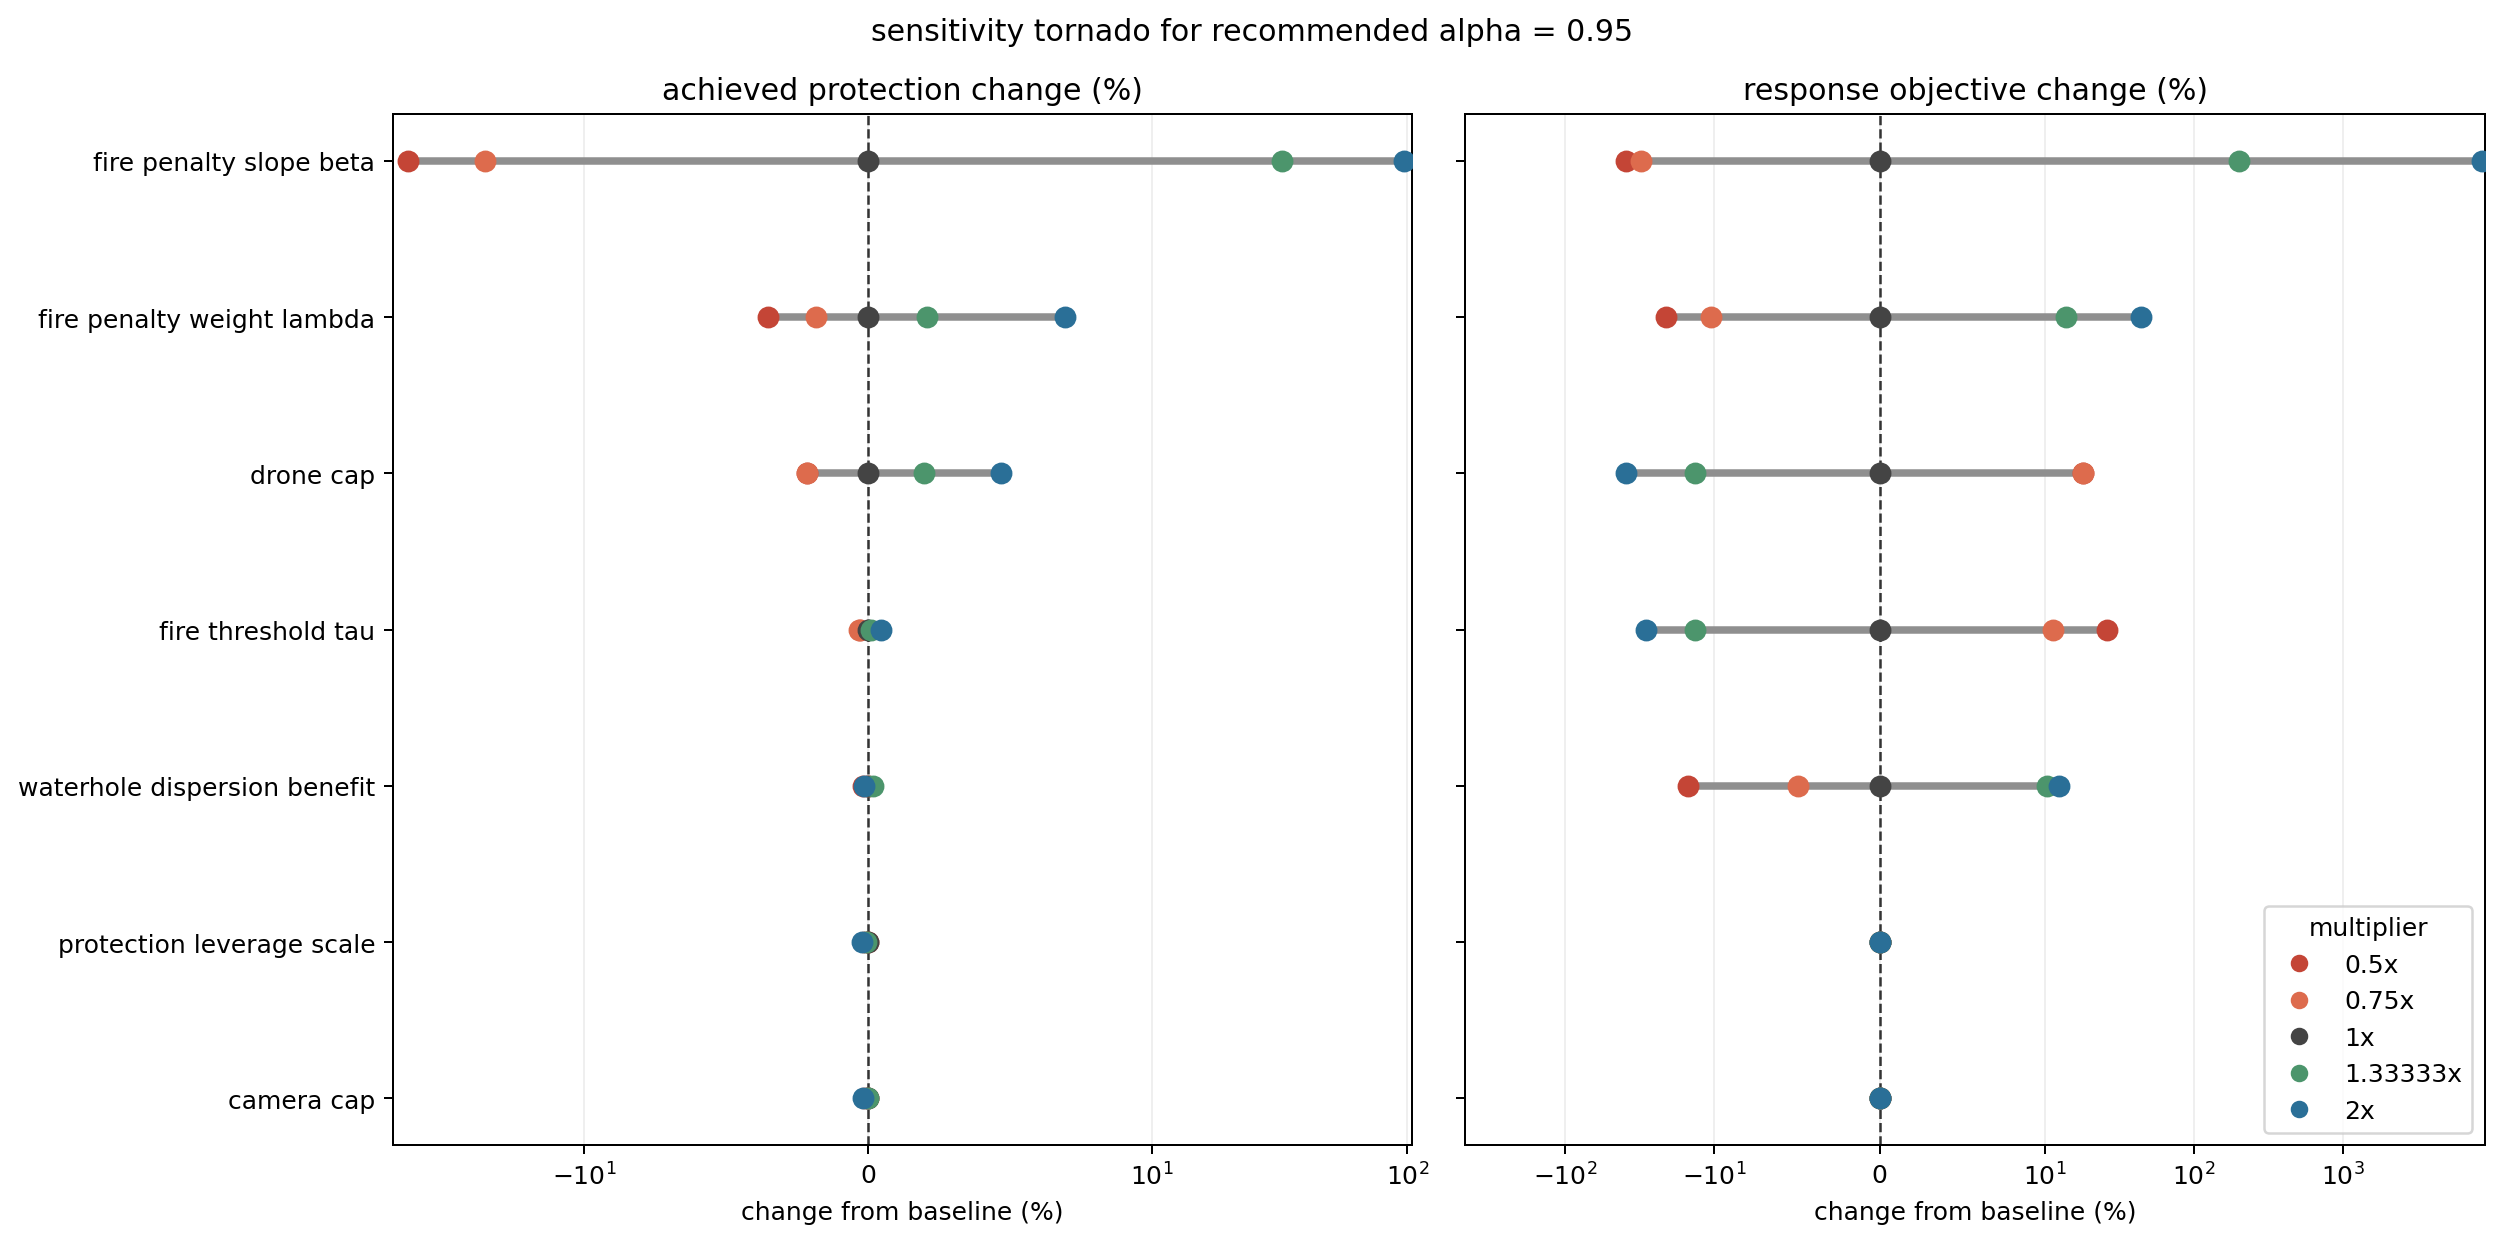
\includegraphics[width=0.95\textwidth]{sensitivity_tornado.png}
\caption{Tornado plot for the one-at-a-time sensitivity analysis at the recommended frontier point}
\label{fig:sensitivity_tornado}
\end{figure}

The tornado plot reports the span of percent changes for
\[
\%\Delta P
\quad\text{and}\quad
\%\Delta R.
\]

\subsection{What the Tornado Plot Shows}

\subsubsection{Fire Penalty Slope \texorpdfstring{$\beta^{\mathrm{fire}}$}{beta fire}}

The dominant parameter is $\beta^{\mathrm{fire}}$:
\[
\%\Delta P \in [-0.17\%,\;0.16\%],
\]
\[
\%\Delta R \in [-39.4\%,\;8604.4\%].
\]
Protection is nearly unchanged, but the response objective is extremely sensitive to the fire-delay slope.

\subsubsection{Drone Cap \texorpdfstring{$\bar{x}^{\mathrm{drone}}$}{drone cap}}

The second-most influential parameter is the drone cap. At $m=0.5$, the selected drone count falls from
\[
n^{\mathrm{drone}}_0 = 3
\quad\text{to}\quad
n^{\mathrm{drone}} = 2,
\]
with
\[
\%\Delta P \approx -2.16\%,
\qquad
\%\Delta R \approx +17.94\%,
\qquad
\%\Delta \bar{t} \approx +6.32\%.
\]

At $m=2.0$, the model expands to
\[
n^{\mathrm{drone}} = 6,
\]
\[
\%\Delta P \approx +4.71\%,
\qquad
\%\Delta R \approx -39.44\%,
\qquad
\%\Delta \bar{t} \approx -23.65\%.
\]
Drone capacity is therefore the strongest actionable deployment lever.

\subsubsection{Camera Cap \texorpdfstring{$\bar{x}^{\mathrm{cam}}$}{camera cap}}

The camera cap mainly affects protection:
\[
\%\Delta R \approx 0
\quad\text{throughout the full tested range.}
\]
\[
\%\Delta P \in [-0.30\%,\;0.47\%].
\]

\subsubsection{Protection Leverage Scale}

The protection leverage scale mostly rescales protection:
\[
\%\Delta R \approx 0,
\qquad
\%\Delta \bar{t} \approx 0.
\]
\[
\%\Delta P \in [-48.81\%,\;97.44\%].
\]

\subsubsection{Waterhole Dispersion Benefit}

The waterhole dispersion benefit has moderate, mixed effects:
\[
\%\Delta P \in [-3.53\%,\;6.94\%],
\qquad
\%\Delta R \in [-15.01\%,\;12.35\%].
\]

\subsubsection{Fire Weight \texorpdfstring{$\lambda^{\mathrm{fire}}$}{lambda fire} and Fire Threshold \texorpdfstring{$\tau^{\mathrm{fire}}$}{tau fire}}

The remaining fire parameters also act primarily through response. For the fire weight,
\[
\%\Delta R \in [-21.03\%,\;44.18\%],
\]
while for the threshold time,
\[
\%\Delta R \in [-28.85\%,\;26.26\%].
\]

In contrast, their protection effects stay very small in magnitude:
\[
|\%\Delta P| < 0.21\%
\]
across the full tested range.

\subsection{Interpretation}

Three conclusions follow. First, the model is most sensitive to wildfire-penalty calibration, especially $\beta^{\mathrm{fire}}$. Second, among operational levers, the drone cap has the strongest effect on both protection and response. Third, some parameters mainly rescale scores rather than changing deployments, most clearly the protection leverage scale. The current recommendation is therefore relatively robust to moderate camera and intervention-value changes, but much less robust to fire calibration and drone capacity.
